\documentclass[11pt]{article}

\usepackage[margin=1in]{geometry}
\usepackage{mathptmx}          % Times New Roman
\usepackage[utf8]{inputenc}
\usepackage[T1]{fontenc}
\usepackage{hyperref}
\usepackage{url}
\usepackage{booktabs}
\usepackage{amsfonts}
\usepackage{amsmath}
\usepackage{microtype}
\usepackage{xcolor}
\usepackage{graphicx}
\graphicspath{{./}{../final/}}
\usepackage{subcaption}
\usepackage{multirow}
\usepackage{float}
\usepackage{parskip}           % space between paragraphs instead of indent
\usepackage{titlesec}

\titlespacing*{\section}{0pt}{14pt}{6pt}
\titlespacing*{\subsection}{0pt}{10pt}{4pt}
\titlespacing*{\subsubsection}{0pt}{8pt}{3pt}

\title{Financial Transaction Category Classification}

\author{%
  Ian Hock \quad Jaden Ong \quad Justin Pelak \quad Sawyer Jones \\[4pt]
  San Diego State University%
}

\begin{document}

\maketitle

\begin{abstract}
This project applies machine learning to classify personal financial transactions into spending categories such as Groceries, Restaurants, Utilities, and Shopping. We use the Personal Transactions dataset, which contains merchant descriptions, transaction amounts, account types, and debit/credit labels. After filtering out 10,000 augmented noise rows with scrambled labels, we work with 791 cleanly labeled transactions across 18 categories. Features are built from TF-IDF on the transaction description, a log-scaled transaction amount, and one-hot encoded categorical fields, producing a 92-dimensional sparse feature matrix. We train and compare four models: Logistic Regression, Support Vector Machine (LinearSVC), a Multi-Layer Perceptron (MLP), and K-Nearest Neighbors (KNN). Logistic Regression achieves the best weighted F1-score of 0.9827 at 98.1\% accuracy. SVM performs nearly identically at 0.9817 F1 while training twice as fast. MLP and KNN trail at 0.9296 and 0.9643 respectively, which we attribute to the small training set size. Results show that for this kind of text-heavy classification task, simpler linear models are hard to beat when descriptions are distinctive enough.
\end{abstract}

\section{Introduction}

\subsection{Background}

Automatic transaction categorization is a core feature of personal finance apps like Mint and YNAB. When a user makes a purchase, the app needs to figure out whether it is a grocery run, a restaurant visit, a subscription payment, or something else. Doing this accurately requires parsing short, often abbreviated merchant names and combining that signal with structured information like transaction amount and account type.

This is a multi-class text classification problem with added numerical and categorical features. The challenge is that merchant names can be ambiguous. A charge from ``Gas Company'' might be a utility bill or a gas station fill-up. ``Roadside Diner'' and ``American Tavern'' both fall under Restaurants but look different in a bag-of-words model. On top of that, some categories appear far less frequently than others, which creates a class imbalance problem.

\subsection{Dataset}

We use the Personal Transactions dataset \cite{dataset}, which contains records with the following fields: User ID, Date, transaction Description, Amount, Transaction Type (debit/credit), Category, and Account Name.

The raw file has 10,806 rows, but closer inspection reveals that 10,000 of them have a missing User ID and randomly shuffled category labels. For example, rows with descriptions like ``Netflix'' are labeled as Coffee Shops, and ``Credit Card Payment'' rows are labeled as Utilities. These are clearly augmented noise rows and cannot be used for supervised learning. We work exclusively with the 806 rows that have valid User IDs and correct labels.

After preprocessing (described in Section~\ref{sec:preprocessing}), we end up with 791 samples across 18 categories. Table~\ref{tab:categories} shows the category distribution. Credit Card Payment is the most common class (143 samples) and Haircut is the smallest (13 samples), giving a roughly 11:1 imbalance ratio.

\begin{table}[H]
  \centering
  \caption{Category distribution in the clean labeled dataset (791 rows).}
  \label{tab:categories}
  \small
  \begin{tabular}{lc|lc}
    \toprule
    Category & Count & Category & Count \\
    \midrule
    Credit Card Payment & 143 & Coffee Shops      & 31 \\
    Groceries           & 105 & Alcohol \& Bars   & 25 \\
    Restaurants         &  81 & Mortgage \& Rent  & 21 \\
    Utilities           &  63 & Internet          & 21 \\
    Shopping            &  60 & Mobile Phone      & 21 \\
    Gas \& Fuel         &  52 & Music             & 21 \\
    Paycheck            &  46 & Movies \& DVDs    & 18 \\
    Home Improvement    &  36 & Auto Insurance    & 18 \\
    Fast Food           &  16 & Haircut           & 13 \\
    \bottomrule
  \end{tabular}
\end{table}

\subsection{Objectives}

\begin{itemize}
  \item Preprocess real-world financial data and identify and handle data quality issues
  \item Build a combined feature representation from text, numerical, and categorical fields
  \item Train and compare four machine learning models on the classification task
  \item Evaluate performance using accuracy, precision, recall, F1-score, and confusion matrices
  \item Understand which model types work best on this kind of structured + text data
\end{itemize}

\section{Methodology}

\subsection{Data Preprocessing}
\label{sec:preprocessing}

The preprocessing pipeline has the following steps:

\textbf{Filtering labeled rows.} We drop all 10,000 rows where User ID is missing, since those rows have scrambled category labels and would introduce incorrect supervision signal.

\textbf{Missing value handling.} Within the 806 labeled rows, we check each column for missing values. Transaction Type and Account Name have no missing entries; Amount and Category also have no missing values in this subset. We still apply defensive fills (median for Amount, ``unknown'' for text fields) to handle edge cases.

\textbf{Duplicate removal.} We remove exact duplicate rows. No duplicates were found in the labeled subset.

\textbf{Text normalization.} Description, Transaction Type, and Account Name are lowercased and stripped of leading/trailing whitespace. This ensures that ``Amazon'' and ``amazon'' are treated as the same token by TF-IDF.

\textbf{Rare category filtering.} Categories with fewer than 10 samples are dropped, since stratified train/test splitting requires at least enough samples per class to appear in both splits. This removes 15 rows, leaving 791 samples.

\subsection{Feature Engineering}

We build three groups of features and concatenate them into a single sparse matrix.

\textbf{TF-IDF on Description.} Transaction descriptions like ``Starbucks'', ``Netflix'', and ``Hardware Store'' carry most of the predictive signal. We apply TF-IDF with unigrams and bigrams (\texttt{ngram\_range=(1,2)}), a vocabulary cap of 2000 terms, sublinear TF scaling, and a minimum document frequency of 2. This produces an 86-feature sparse matrix. The vocabulary cap and \texttt{min\_df=2} help reduce noise from one-off descriptions.

\textbf{Amount.} Transaction amount is log-transformed using $\log(1 + x)$ to reduce the effect of large outliers (e.g., mortgage payments), then standardized with \texttt{StandardScaler}. This adds 1 feature.

\textbf{Categorical features.} Transaction Type (debit or credit) and Account Name (Checking, Platinum Card, Silver Card) are one-hot encoded. These add 5 binary features. Encoding account name is useful because certain account types are associated with specific spending patterns.

The combined feature matrix has shape $(791, 92)$. All three feature groups are stacked using \texttt{scipy.sparse.hstack} to keep memory usage low.

\textbf{Train/test split.} We use a stratified 80/20 split (\texttt{RANDOM\_STATE=42}), giving 632 training samples and 159 test samples. Stratification ensures each class is proportionally represented in both sets.

\subsection{Handling Class Imbalance}

Rather than oversampling (SMOTE) or undersampling, we use \texttt{class\_weight=`balanced'} in all applicable models. This scales each class's loss contribution inversely to its frequency. We chose this approach because the dataset is small (632 training samples) and SMOTE on a high-dimensional sparse TF-IDF matrix can generate synthetic samples that do not meaningfully resemble real transactions.

Figure~\ref{fig:imbalance} shows the training set class distribution.

\begin{figure}[H]
  \centering
  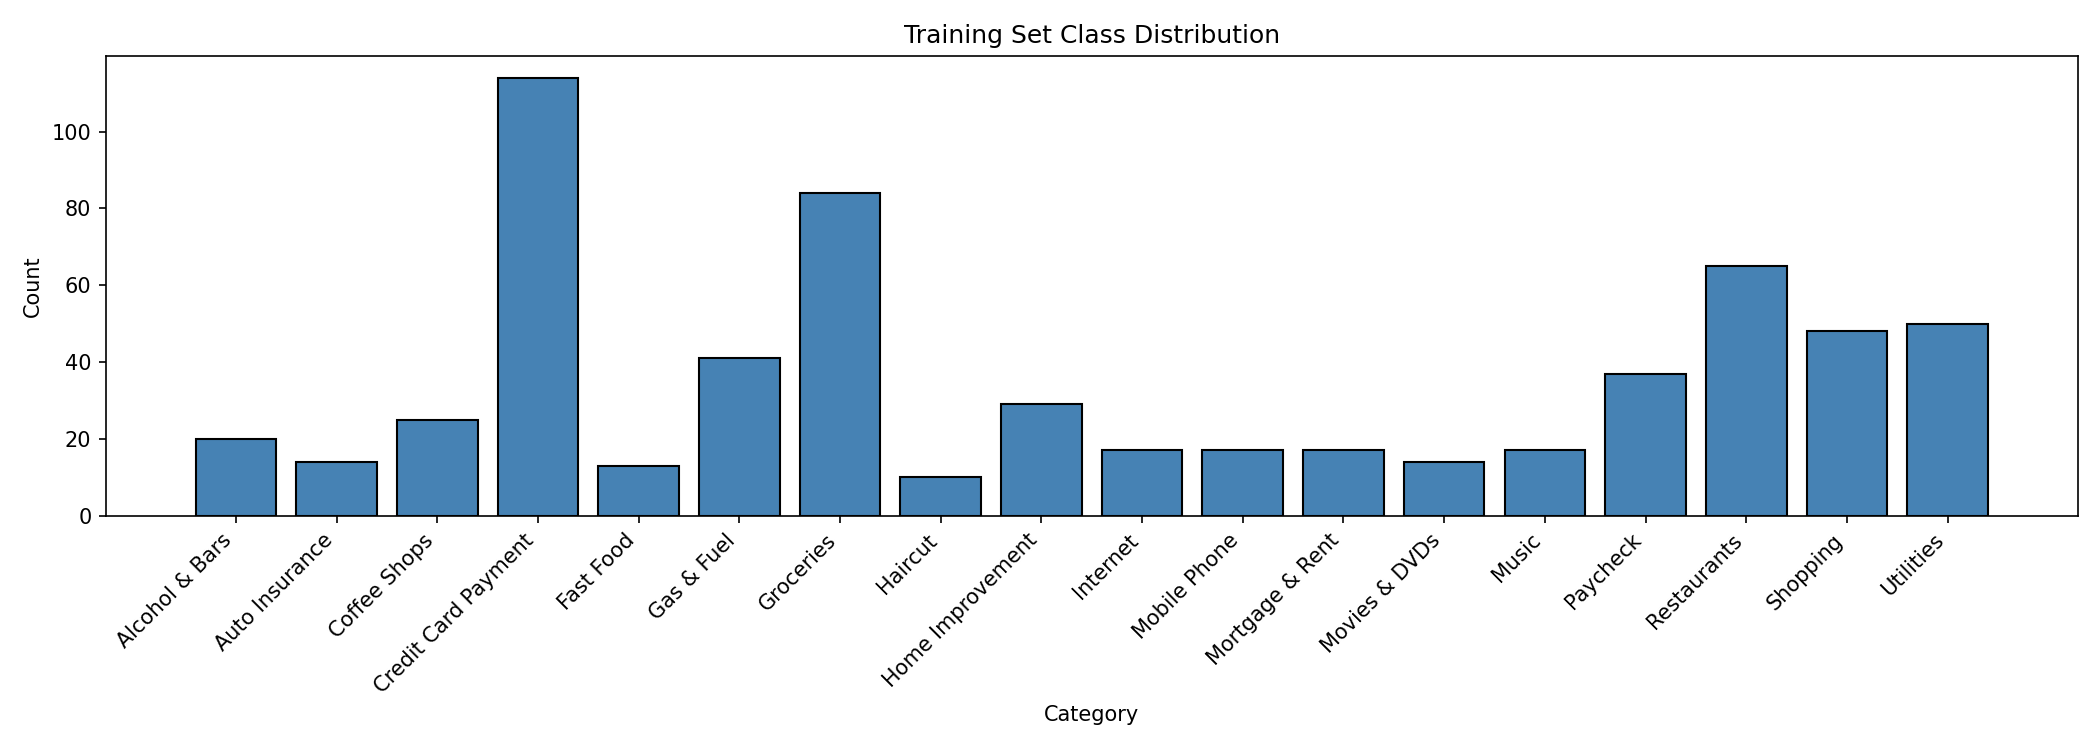
\includegraphics[width=0.85\textwidth]{class_imbalance.png}
  \caption{Training set class distribution. Credit Card Payment is the dominant class at roughly 11x the size of Haircut.}
  \label{fig:imbalance}
\end{figure}

\subsection{Models}

\subsubsection{Logistic Regression}
\textit{(Sawyer Jones)}

Logistic Regression is our baseline. It is a linear classifier that learns a weight vector per class and classifies by taking the argmax of class scores. It is fast, interpretable (we can inspect which TF-IDF tokens most drive each class prediction), and known to perform well on high-dimensional sparse text features. We use the \texttt{lbfgs} solver with L2 regularization (\texttt{C=1.0}) and \texttt{class\_weight=`balanced'}.

\subsubsection{Support Vector Machine (LinearSVC)}
\textit{(Jaden Ong)}

LinearSVC finds a maximum-margin separating hyperplane between classes using a one-vs-rest strategy. Like Logistic Regression, it handles high-dimensional sparse input well. The key hyperparameter is the regularization constant $C$, which controls the trade-off between margin width and training error. We tune $C$ using 5-fold cross-validation over $\{0.01, 0.05, 0.1, 0.5, 1.0, 5.0, 10.0\}$ and select the value that maximizes weighted F1.

\subsubsection{Neural Network (MLP)}
\textit{(Ian Hock)}

We train a three-layer MLP with hidden sizes $(256, 128, 64)$, ReLU activations, and the Adam optimizer. L2 regularization is applied via \texttt{alpha=1e-4}. The learning rate is set to adaptive, which reduces it when training loss stops improving. To avoid overfitting on the small dataset, we use early stopping with a 10\% validation split and a patience of 20 epochs. The MLP is the only model that can learn non-linear interactions between features, so it serves as a test of whether the task actually requires non-linear modeling.

\subsubsection{K-Nearest Neighbors (KNN)}
\textit{(Justin Pelak)}

KNN assigns a label by majority vote among the $K$ nearest training points. Since we are working with sparse TF-IDF vectors, we use cosine distance, which is more meaningful than Euclidean distance in high-dimensional sparse spaces. We tune $K$ via 5-fold cross-validation over $\{1, 3, 5, 7, 10, 15, 20\}$.

\subsection{Hyperparameter Tuning}

For SVM, the cross-validation F1 scores over the $C$ range are shown in Figure~\ref{fig:svm_tune}. For KNN, the CV scores over $K$ values are shown in Figure~\ref{fig:knn_tune}. LR was not tuned beyond \texttt{C=1.0} since it already performed well, and MLP hyperparameters were set based on prior experiments with the hidden layer sizes and alpha.

\begin{figure}[H]
  \centering
  \begin{subfigure}[b]{0.48\textwidth}
    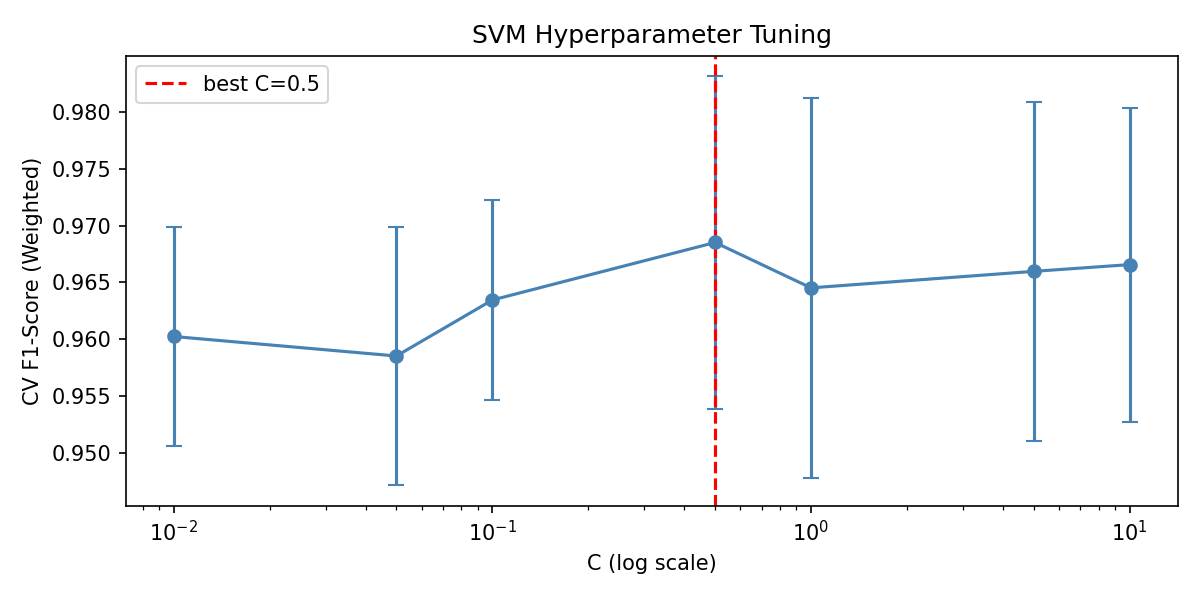
\includegraphics[width=\textwidth]{svm_hyperparameter_tuning.png}
    \caption{SVM: CV F1 vs. regularization parameter $C$.}
    \label{fig:svm_tune}
  \end{subfigure}
  \hfill
  \begin{subfigure}[b]{0.48\textwidth}
    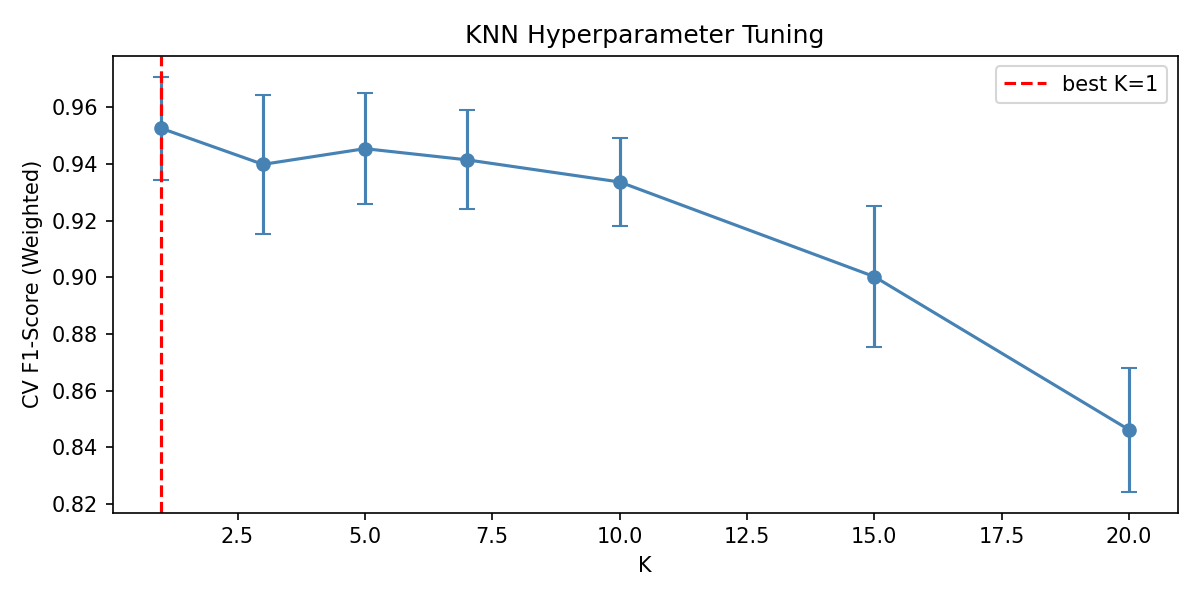
\includegraphics[width=\textwidth]{knn_hyperparameter_tuning.png}
    \caption{KNN: CV F1 vs. number of neighbors $K$.}
    \label{fig:knn_tune}
  \end{subfigure}
  \caption{Hyperparameter tuning curves for SVM and KNN using 5-fold cross-validation on the training set.}
\end{figure}

\section{Results}

\subsection{Performance Metrics}

Table~\ref{tab:results} shows accuracy, weighted precision, recall, and F1-score for all four models on the held-out test set, along with training time.

\begin{table}[H]
  \centering
  \caption{Model performance on the test set (159 samples, 18 classes). All metrics are weighted averages across classes.}
  \label{tab:results}
  \begin{tabular}{lccccr}
    \toprule
    Model & Accuracy & Precision & Recall & F1-Score & Train Time \\
    \midrule
    Logistic Regression  & 0.9811 & 0.9874 & 0.9811 & 0.9827 & 0.04s \\
    SVM (LinearSVC)      & 0.9811 & 0.9852 & 0.9811 & 0.9817 & 0.02s \\
    Neural Network (MLP) & 0.9434 & 0.9233 & 0.9434 & 0.9296 & 0.89s \\
    KNN                  & 0.9623 & 0.9728 & 0.9623 & 0.9643 & 0.00s \\
    \bottomrule
  \end{tabular}
\end{table}

Figure~\ref{fig:comparison} provides a visual comparison of all four metrics across models, and Figure~\ref{fig:time} shows training time.

\begin{figure}[H]
  \centering
  \begin{subfigure}[b]{0.62\textwidth}
    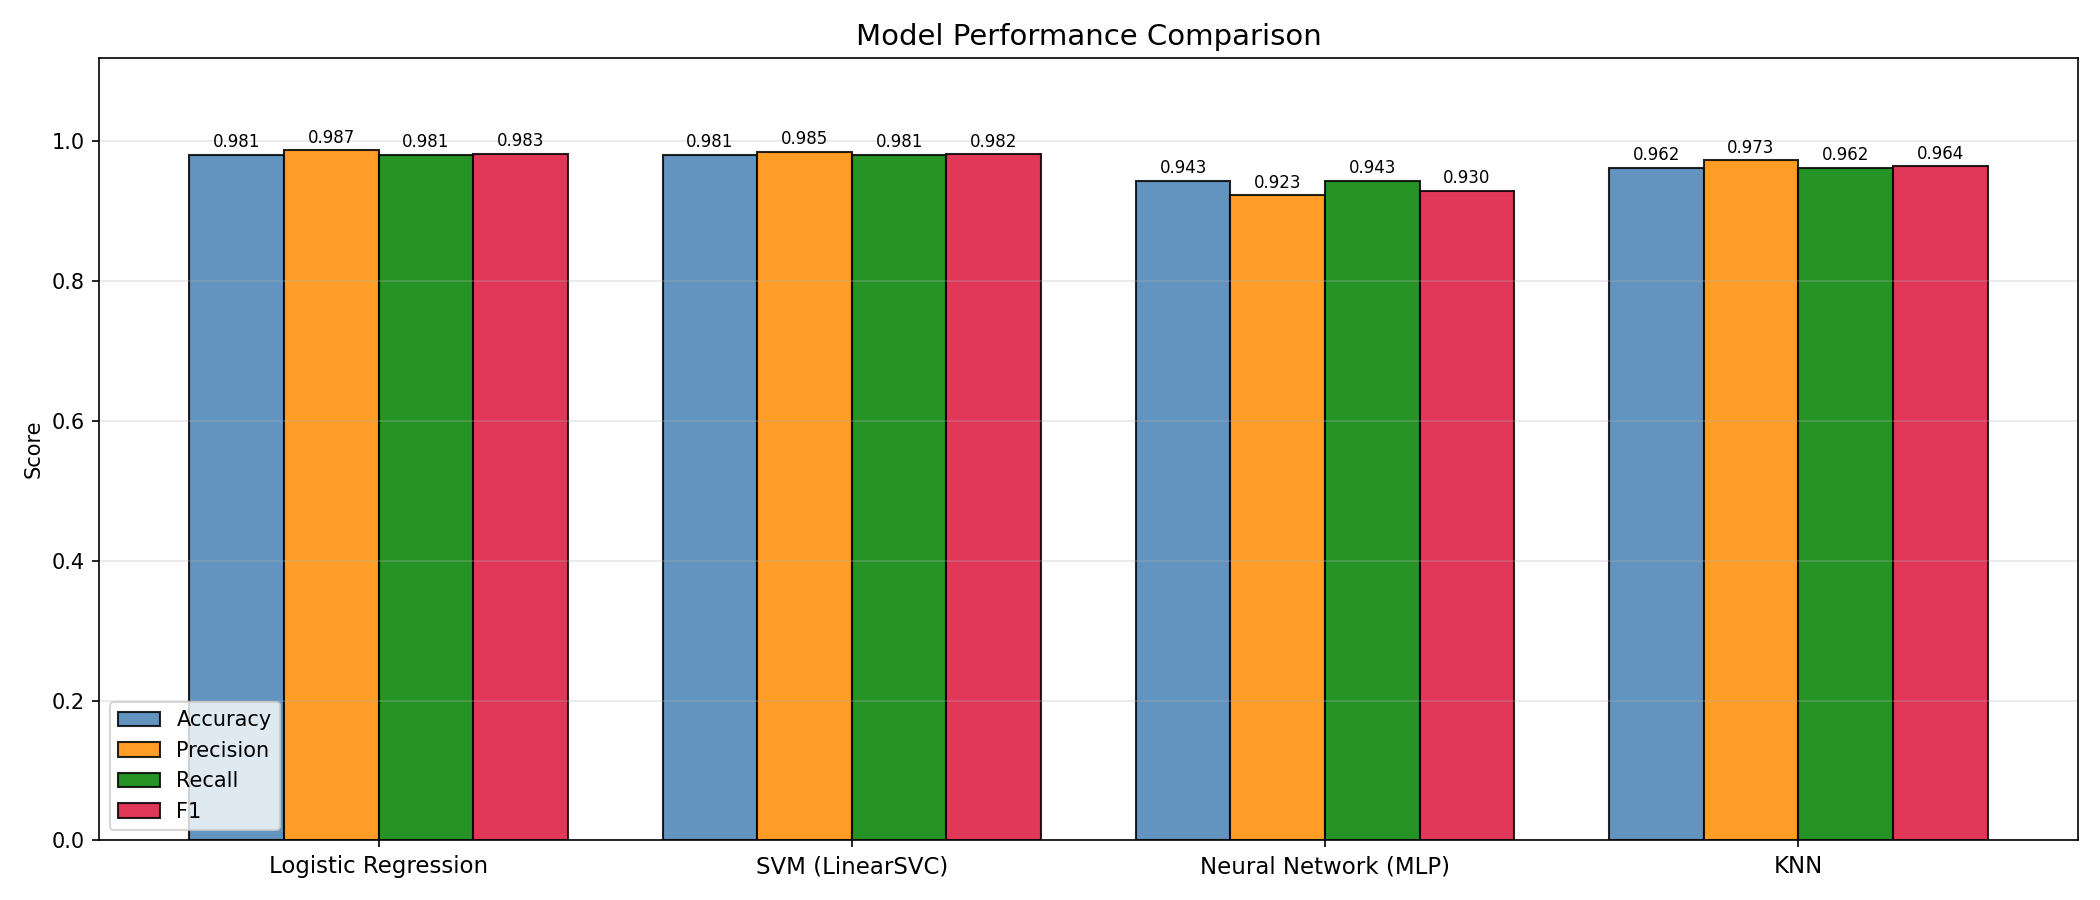
\includegraphics[width=\textwidth]{model_comparison.png}
    \caption{Accuracy, precision, recall, and F1 for each model.}
    \label{fig:comparison}
  \end{subfigure}
  \hfill
  \begin{subfigure}[b]{0.35\textwidth}
    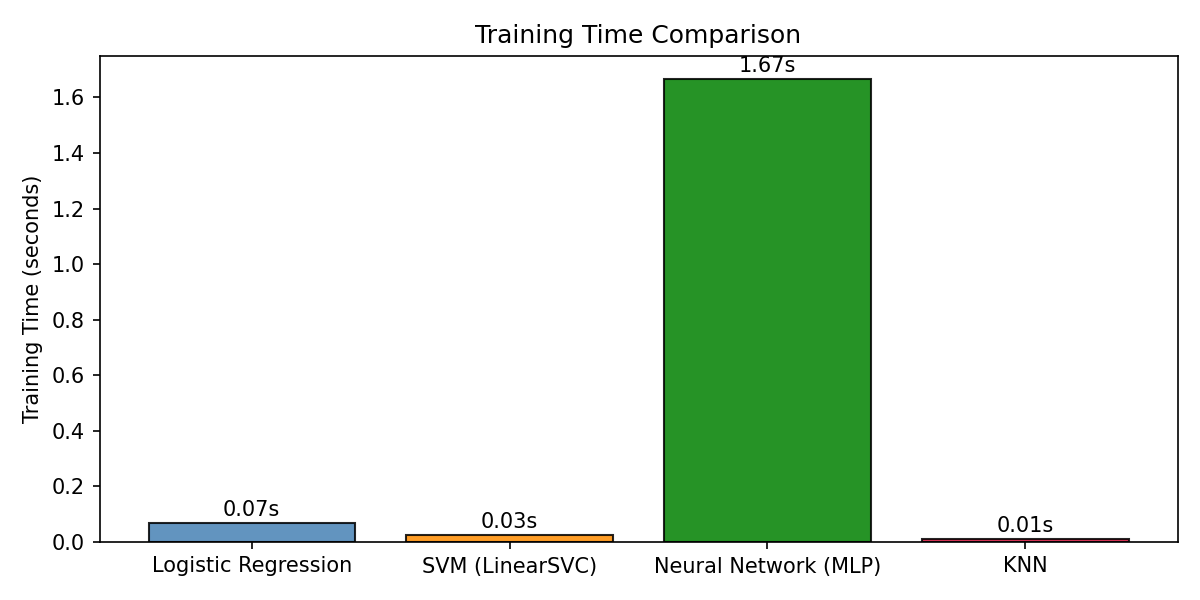
\includegraphics[width=\textwidth]{training_time_comparison.png}
    \caption{Training time in seconds.}
    \label{fig:time}
  \end{subfigure}
  \caption{Model performance and efficiency comparison.}
\end{figure}

\subsection{Confusion Matrices}

Figures~\ref{fig:cm_lr}--\ref{fig:cm_knn} show confusion matrices for each model on the test set.

\begin{figure}[H]
  \centering
  \begin{subfigure}[b]{0.48\textwidth}
    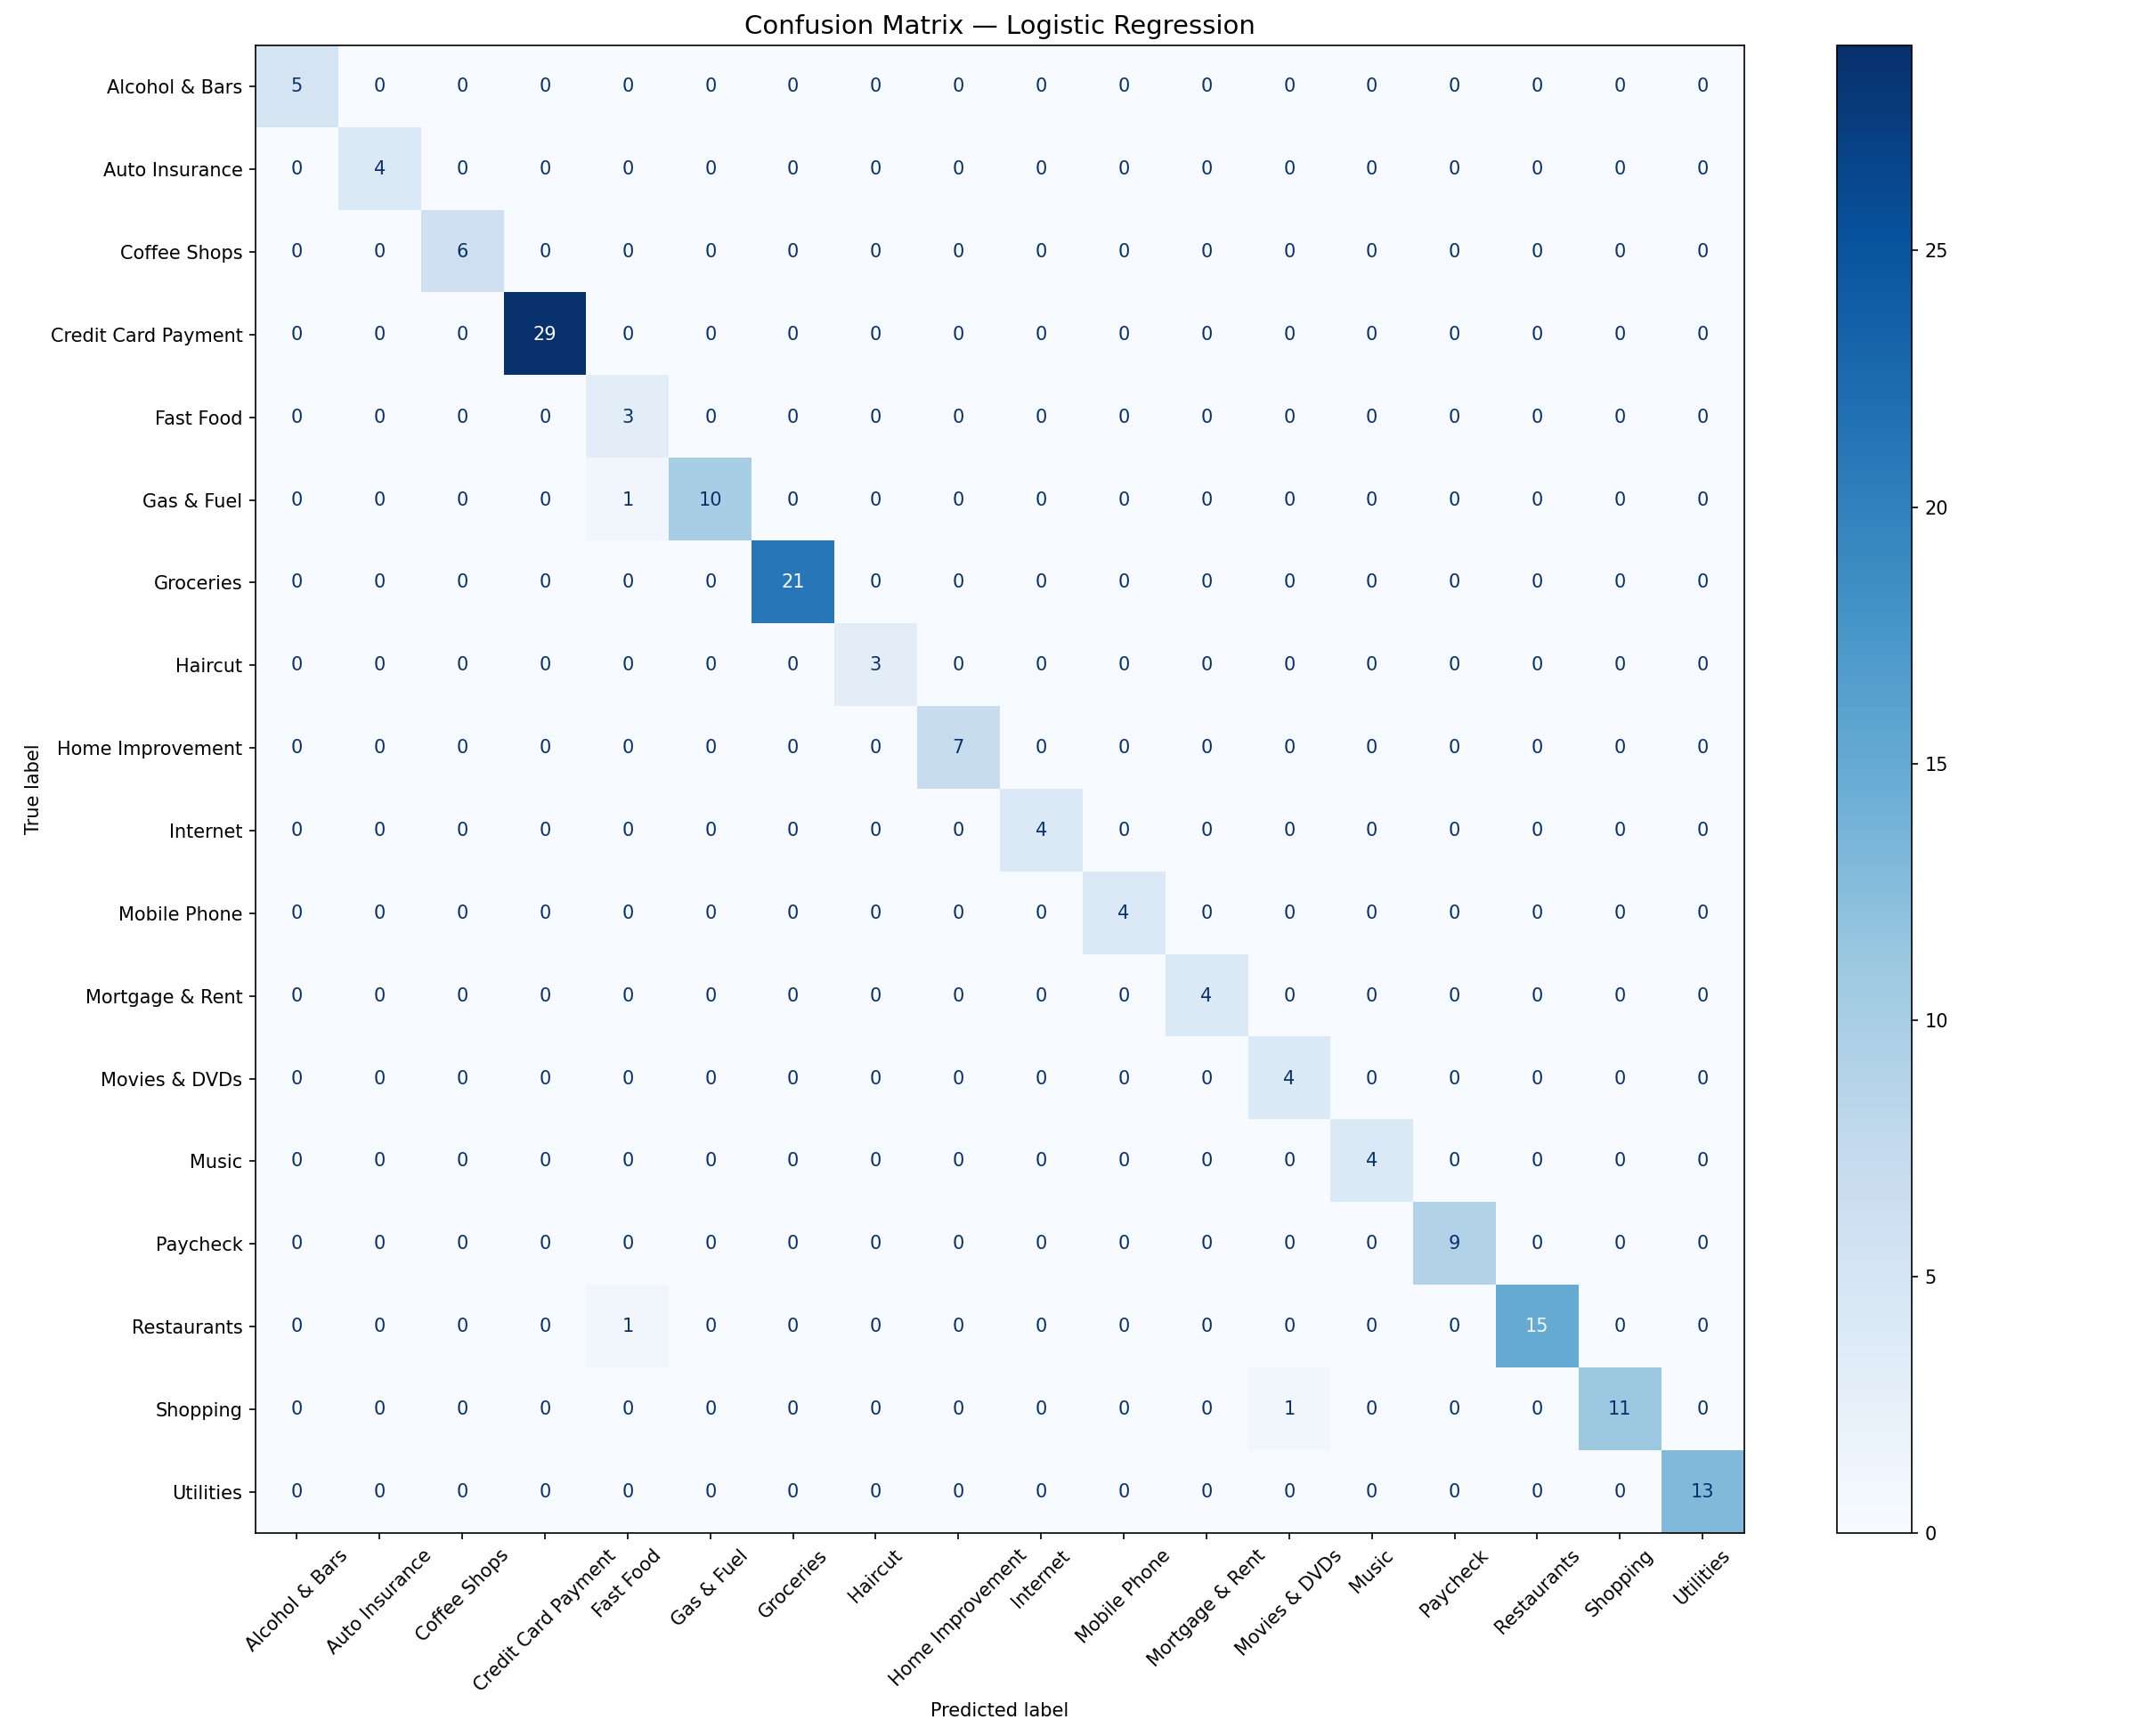
\includegraphics[width=\textwidth,height=0.32\textheight,keepaspectratio]{cm_logistic_regression.png}
    \caption{Logistic Regression}
    \label{fig:cm_lr}
  \end{subfigure}
  \hfill
  \begin{subfigure}[b]{0.48\textwidth}
    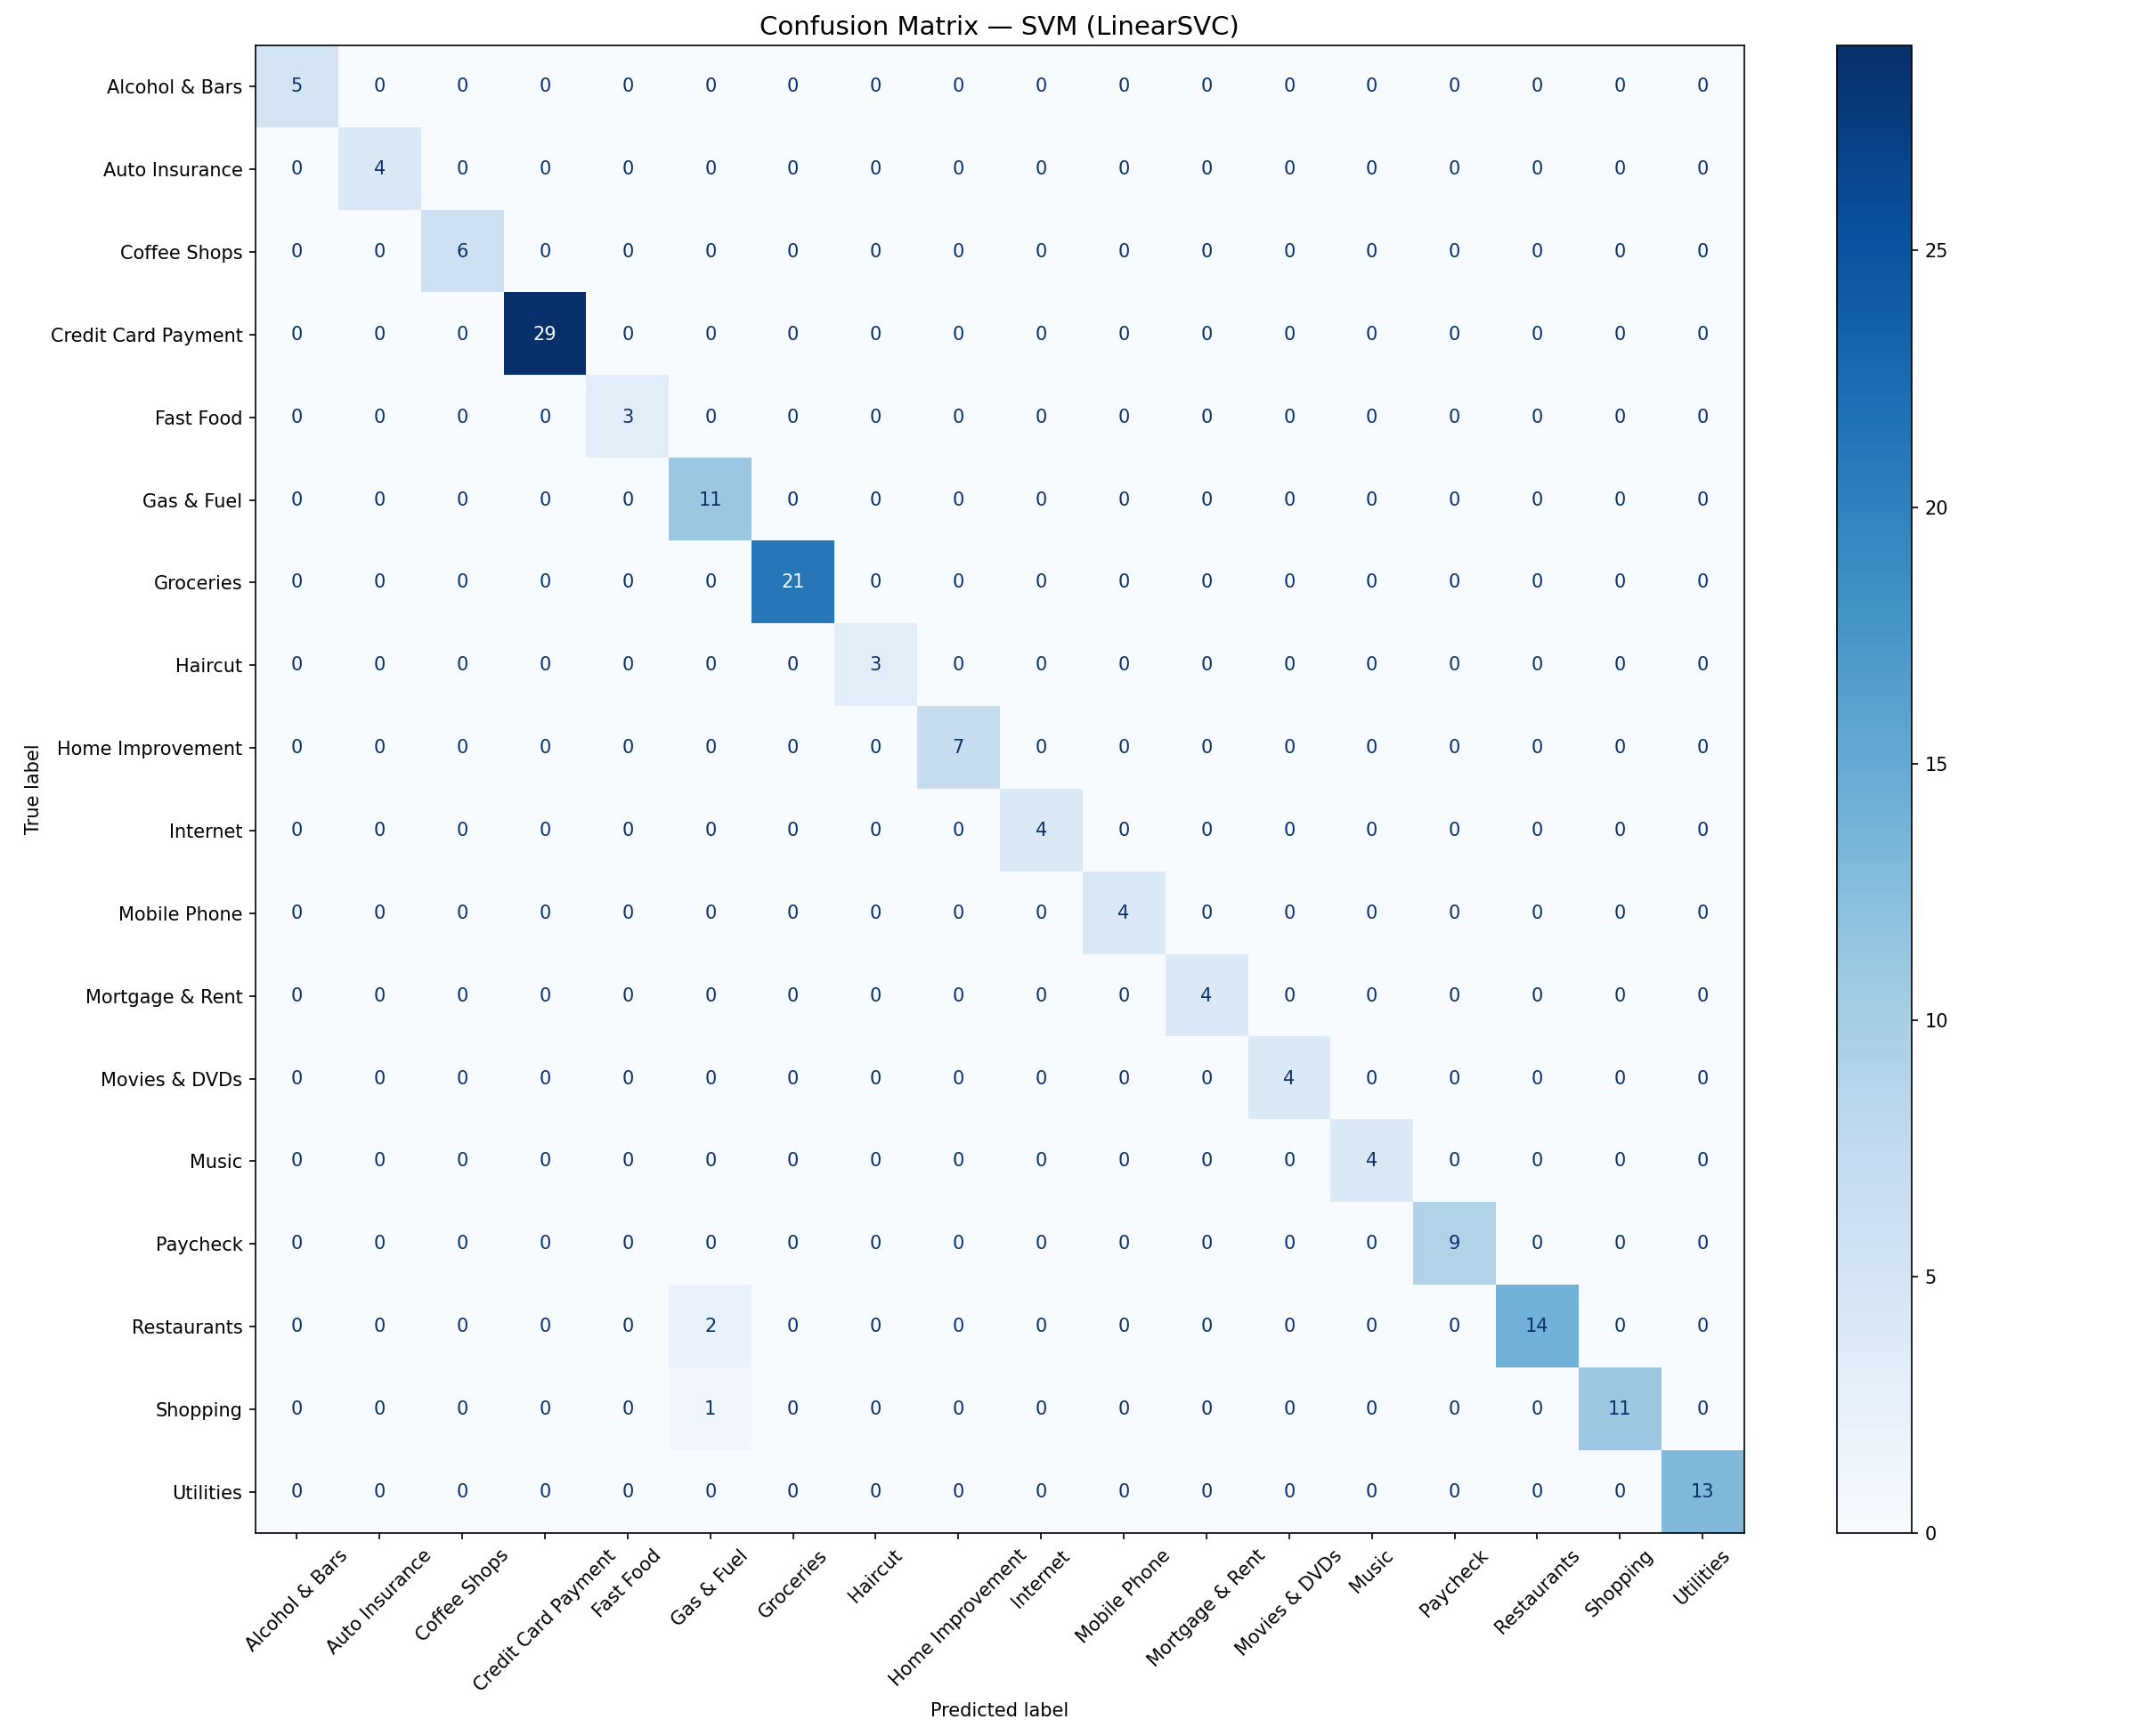
\includegraphics[width=\textwidth,height=0.32\textheight,keepaspectratio]{cm_svm_linearsvc.png}
    \caption{SVM (LinearSVC)}
    \label{fig:cm_svm}
  \end{subfigure}
  \caption{Confusion matrices for the two best-performing models.}
\end{figure}

\begin{figure}[H]
  \centering
  \begin{subfigure}[b]{0.48\textwidth}
    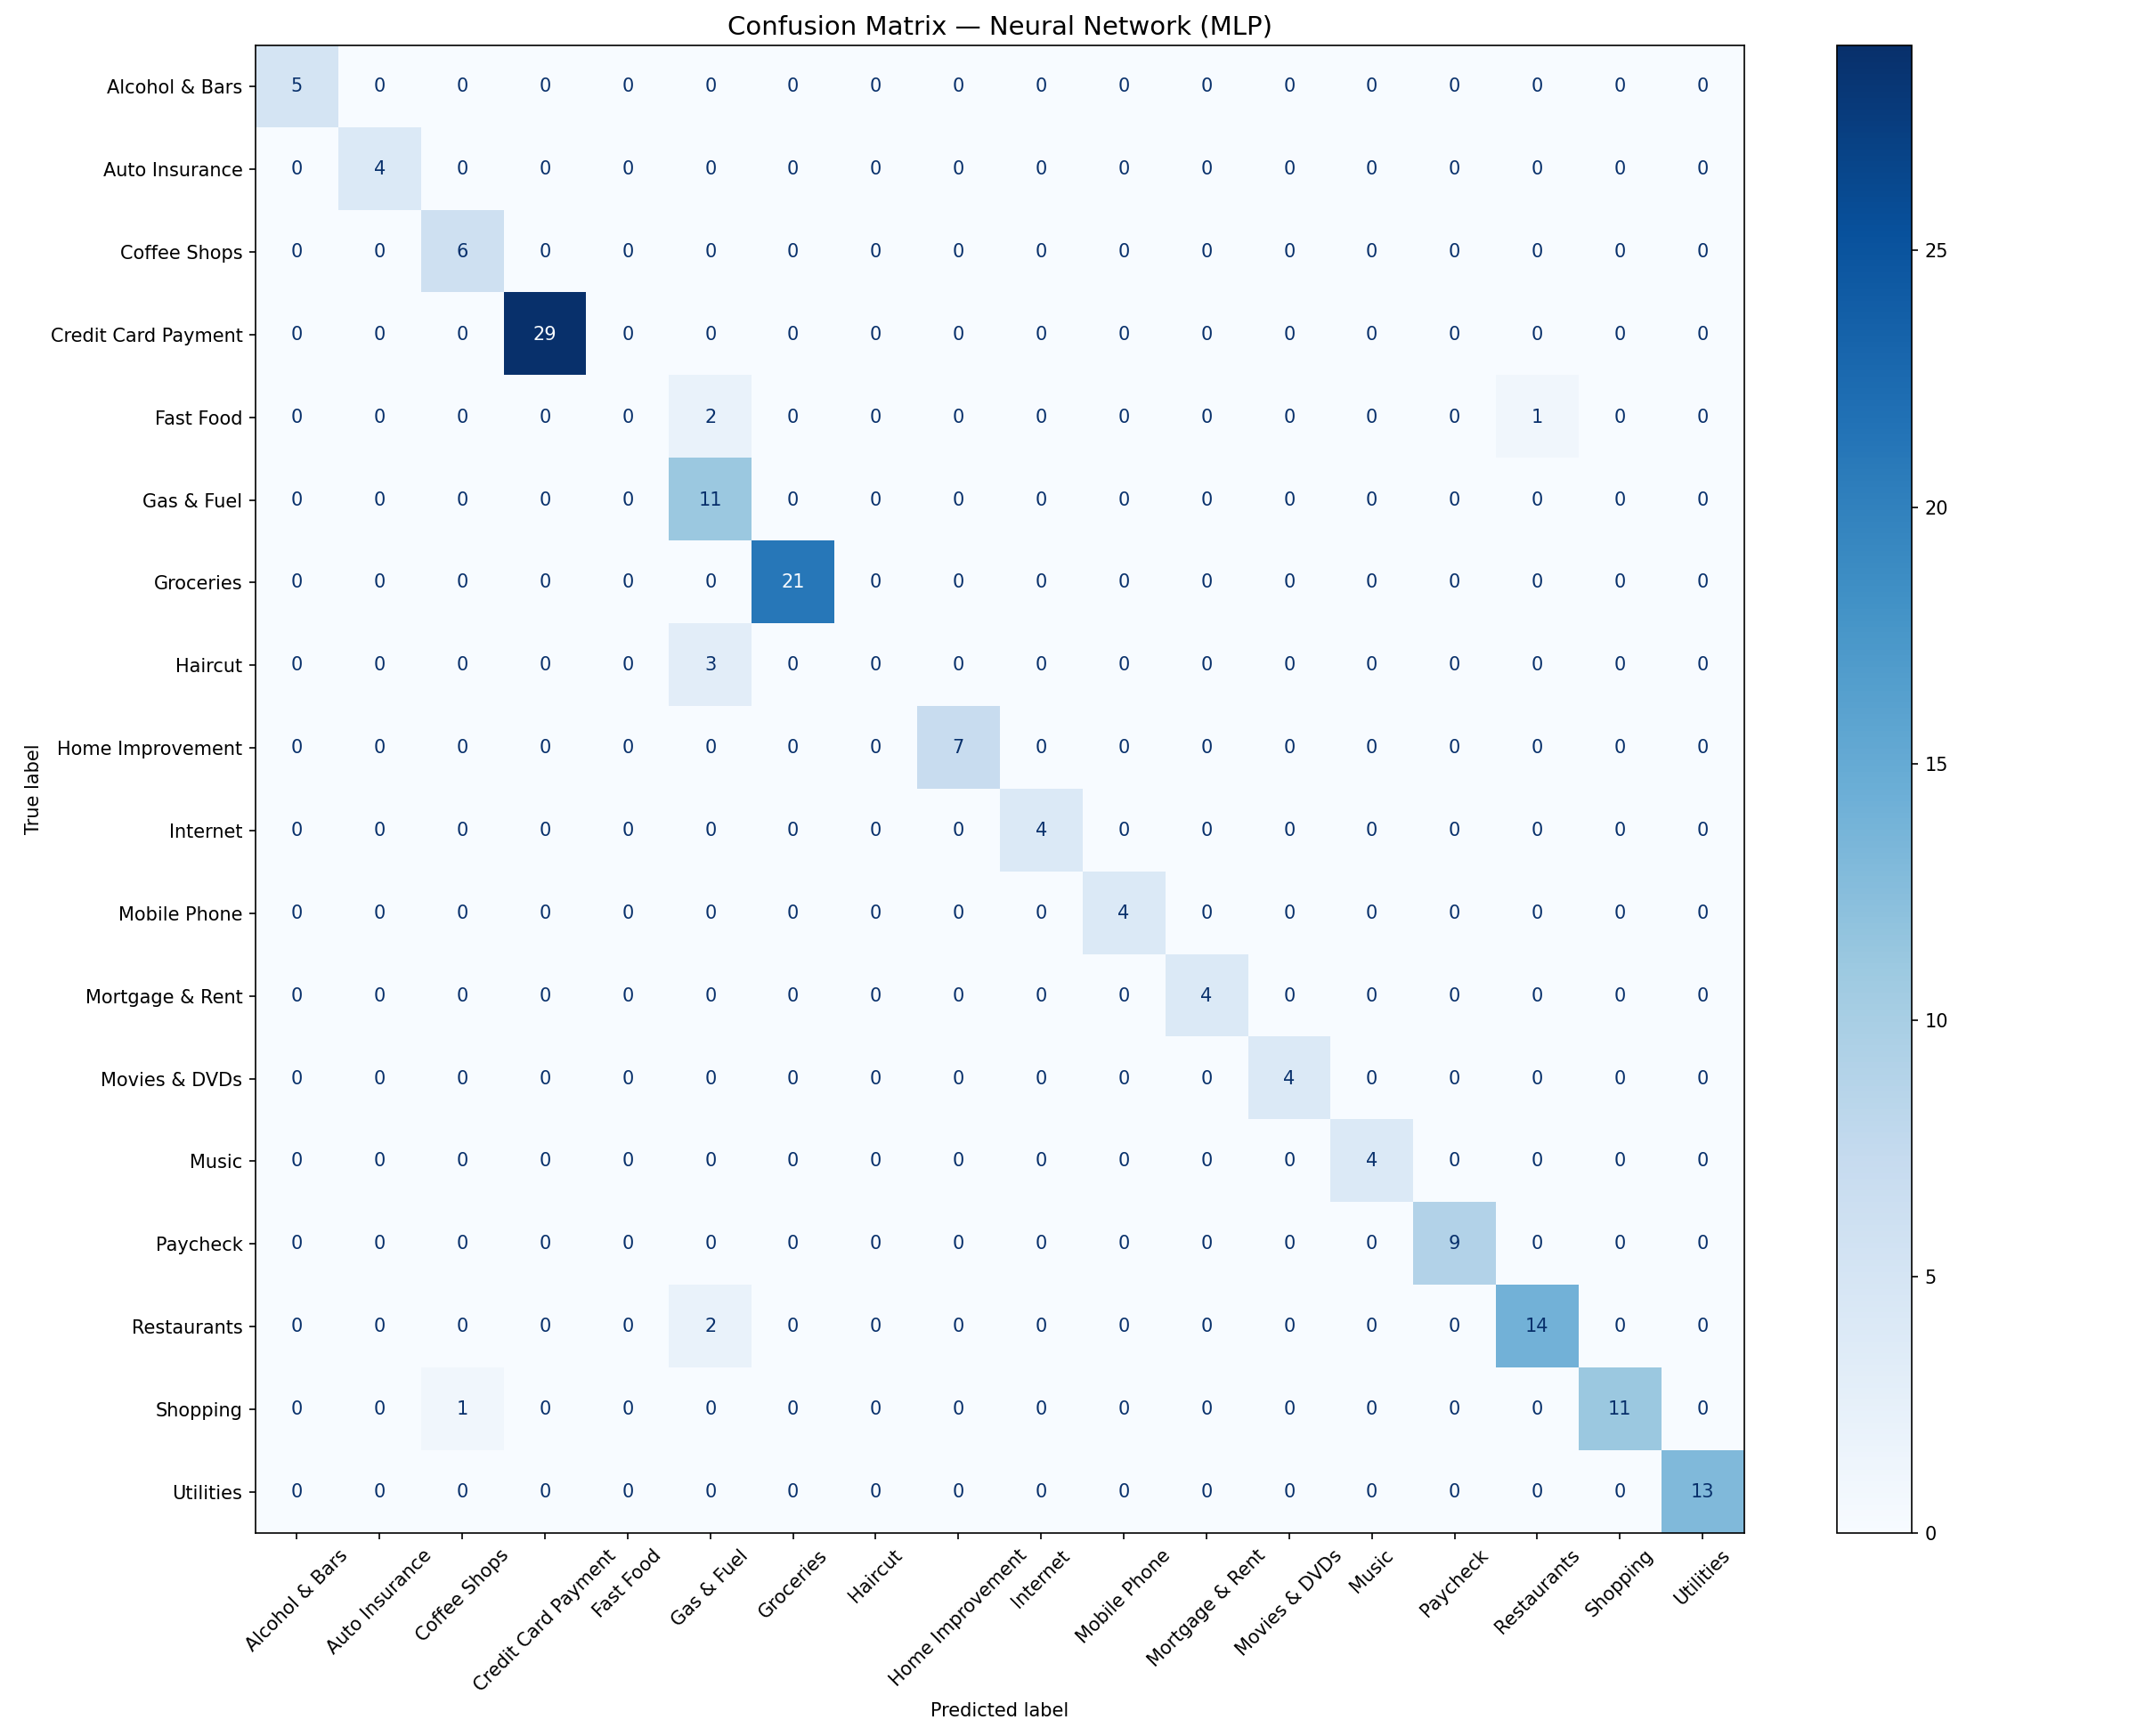
\includegraphics[width=\textwidth,height=0.32\textheight,keepaspectratio]{cm_neural_network_mlp.png}
    \caption{Neural Network (MLP)}
    \label{fig:cm_mlp}
  \end{subfigure}
  \hfill
  \begin{subfigure}[b]{0.48\textwidth}
    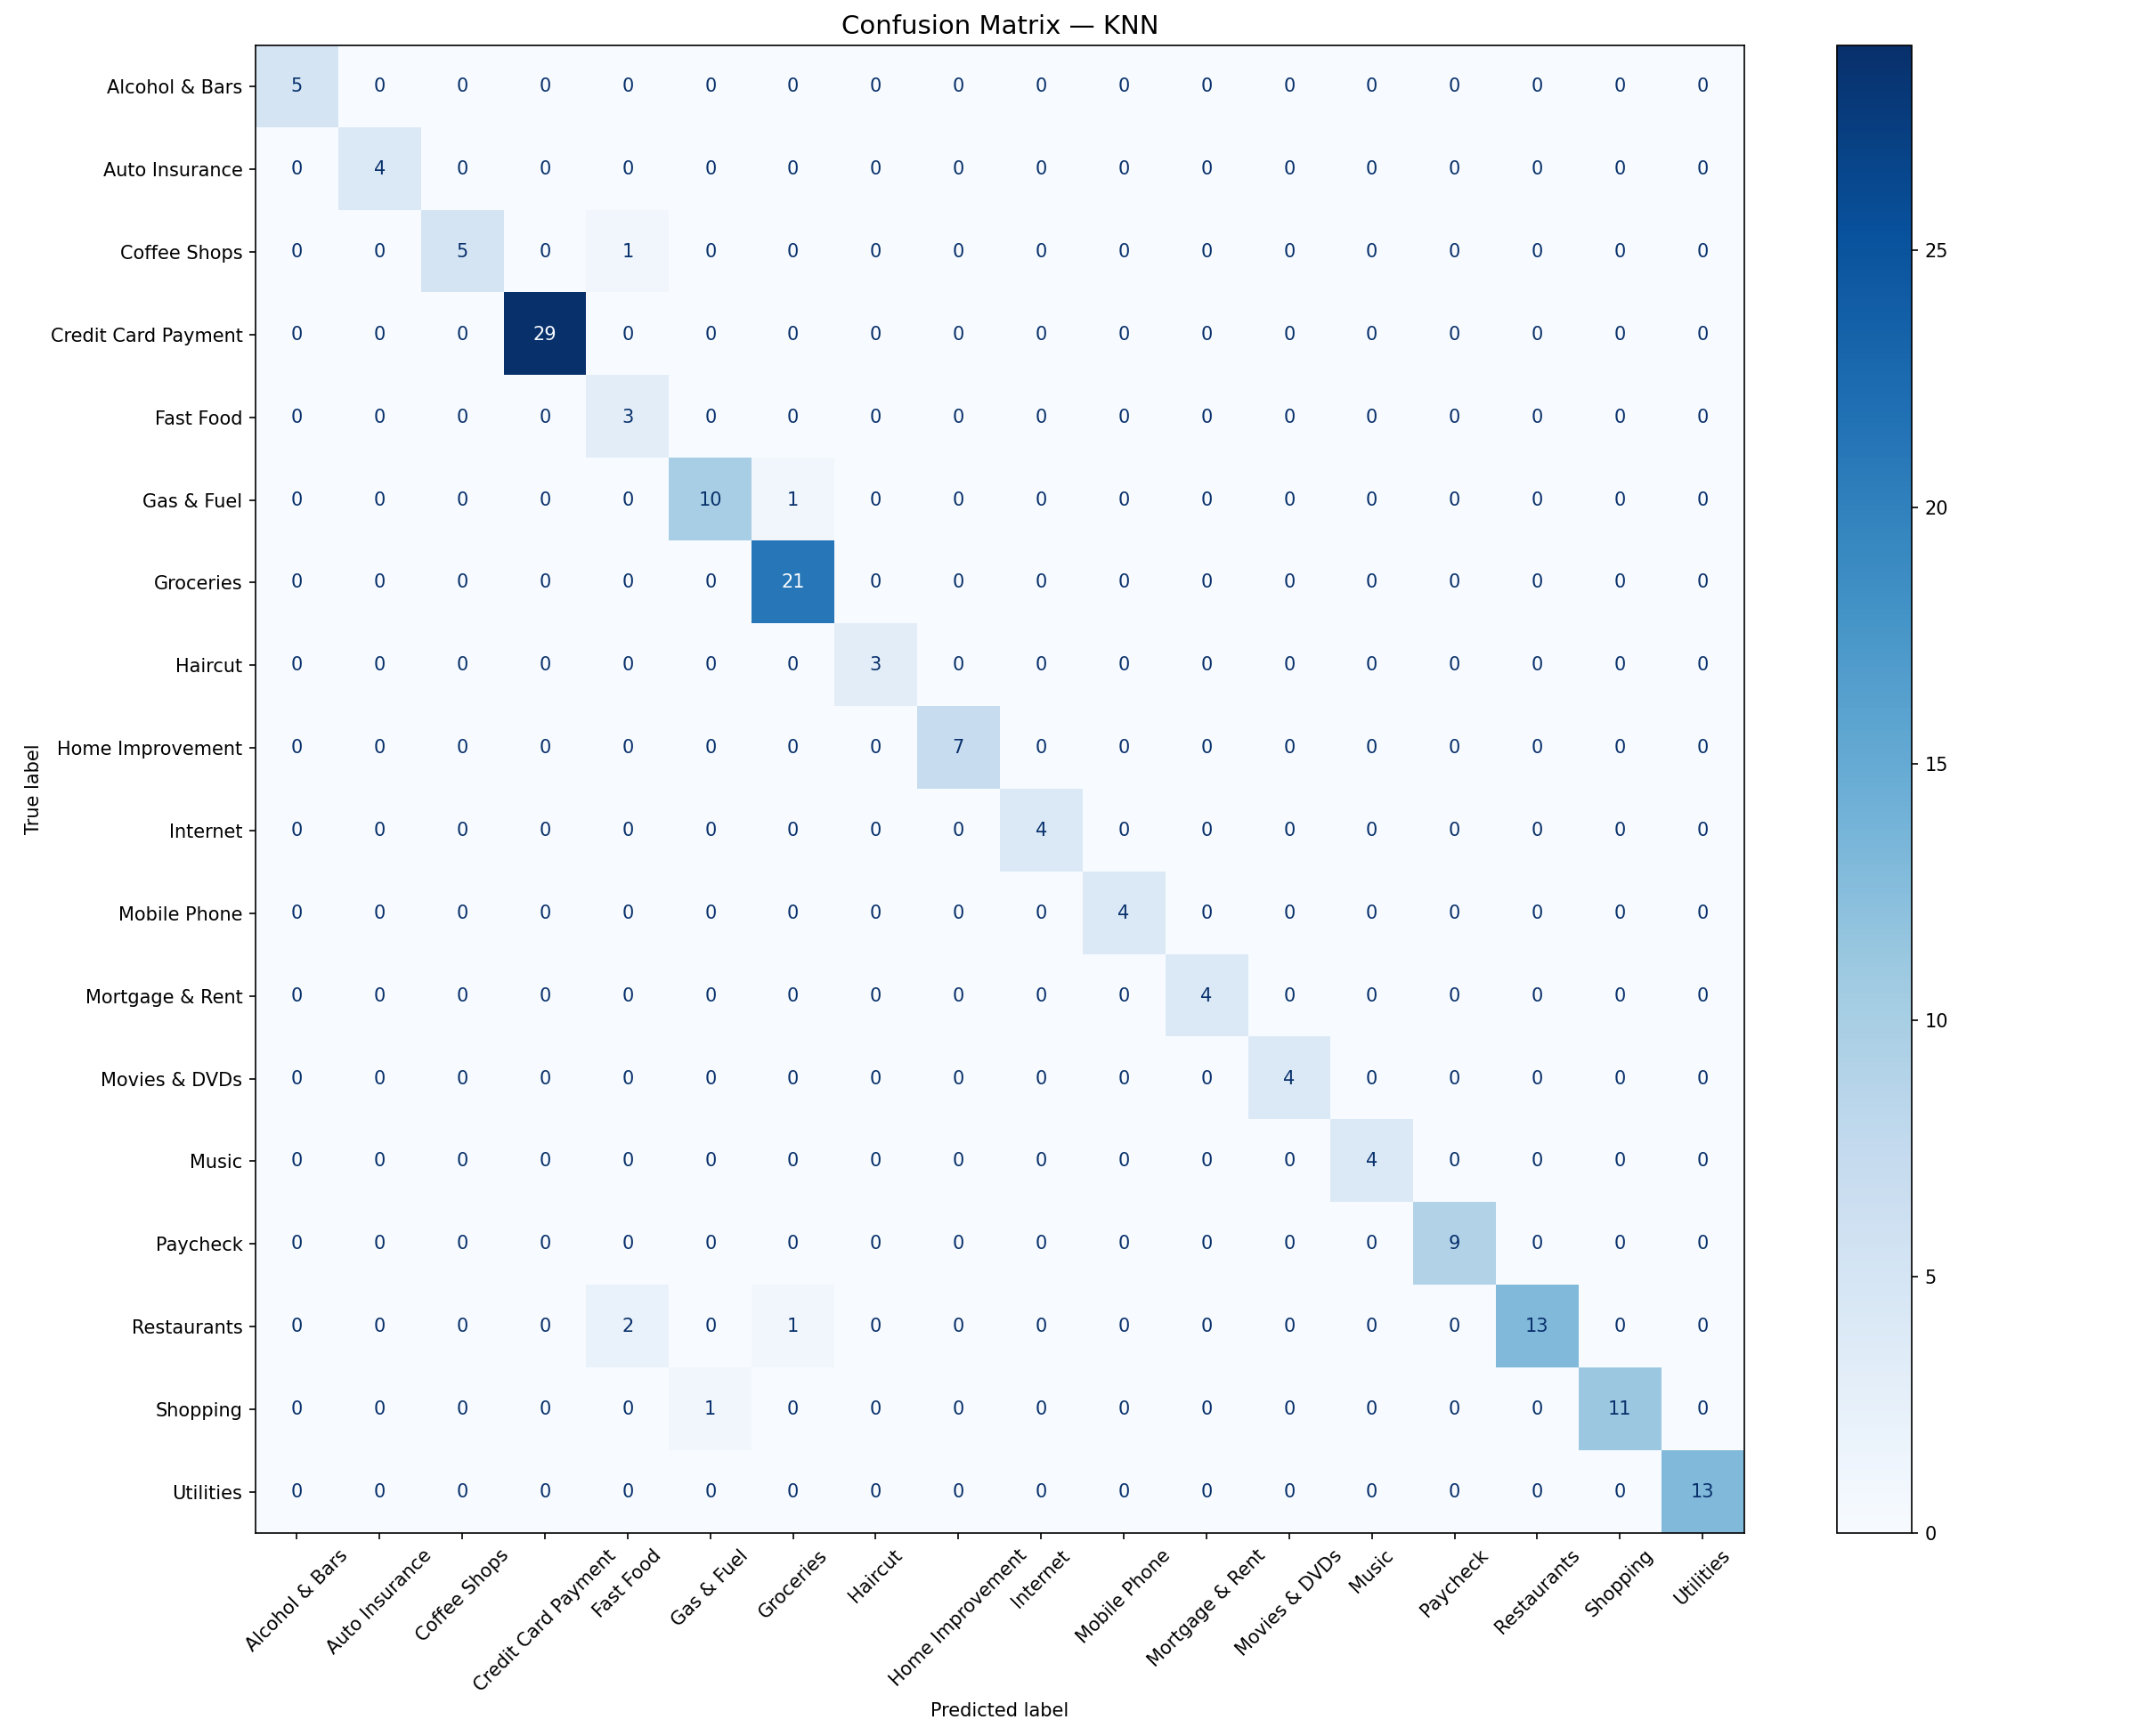
\includegraphics[width=\textwidth,height=0.32\textheight,keepaspectratio]{cm_knn.png}
    \caption{KNN}
    \label{fig:cm_knn}
  \end{subfigure}
  \caption{Confusion matrices for MLP and KNN.}
\end{figure}

\subsection{Per-Class Analysis}

Figure~\ref{fig:heatmap} shows a heatmap of per-class F1-scores for all four models. Most categories reach near-perfect F1 across all models. The categories with the most consistent drops are Gas \& Fuel, Restaurants, and Shopping.

\begin{figure}[H]
  \centering
  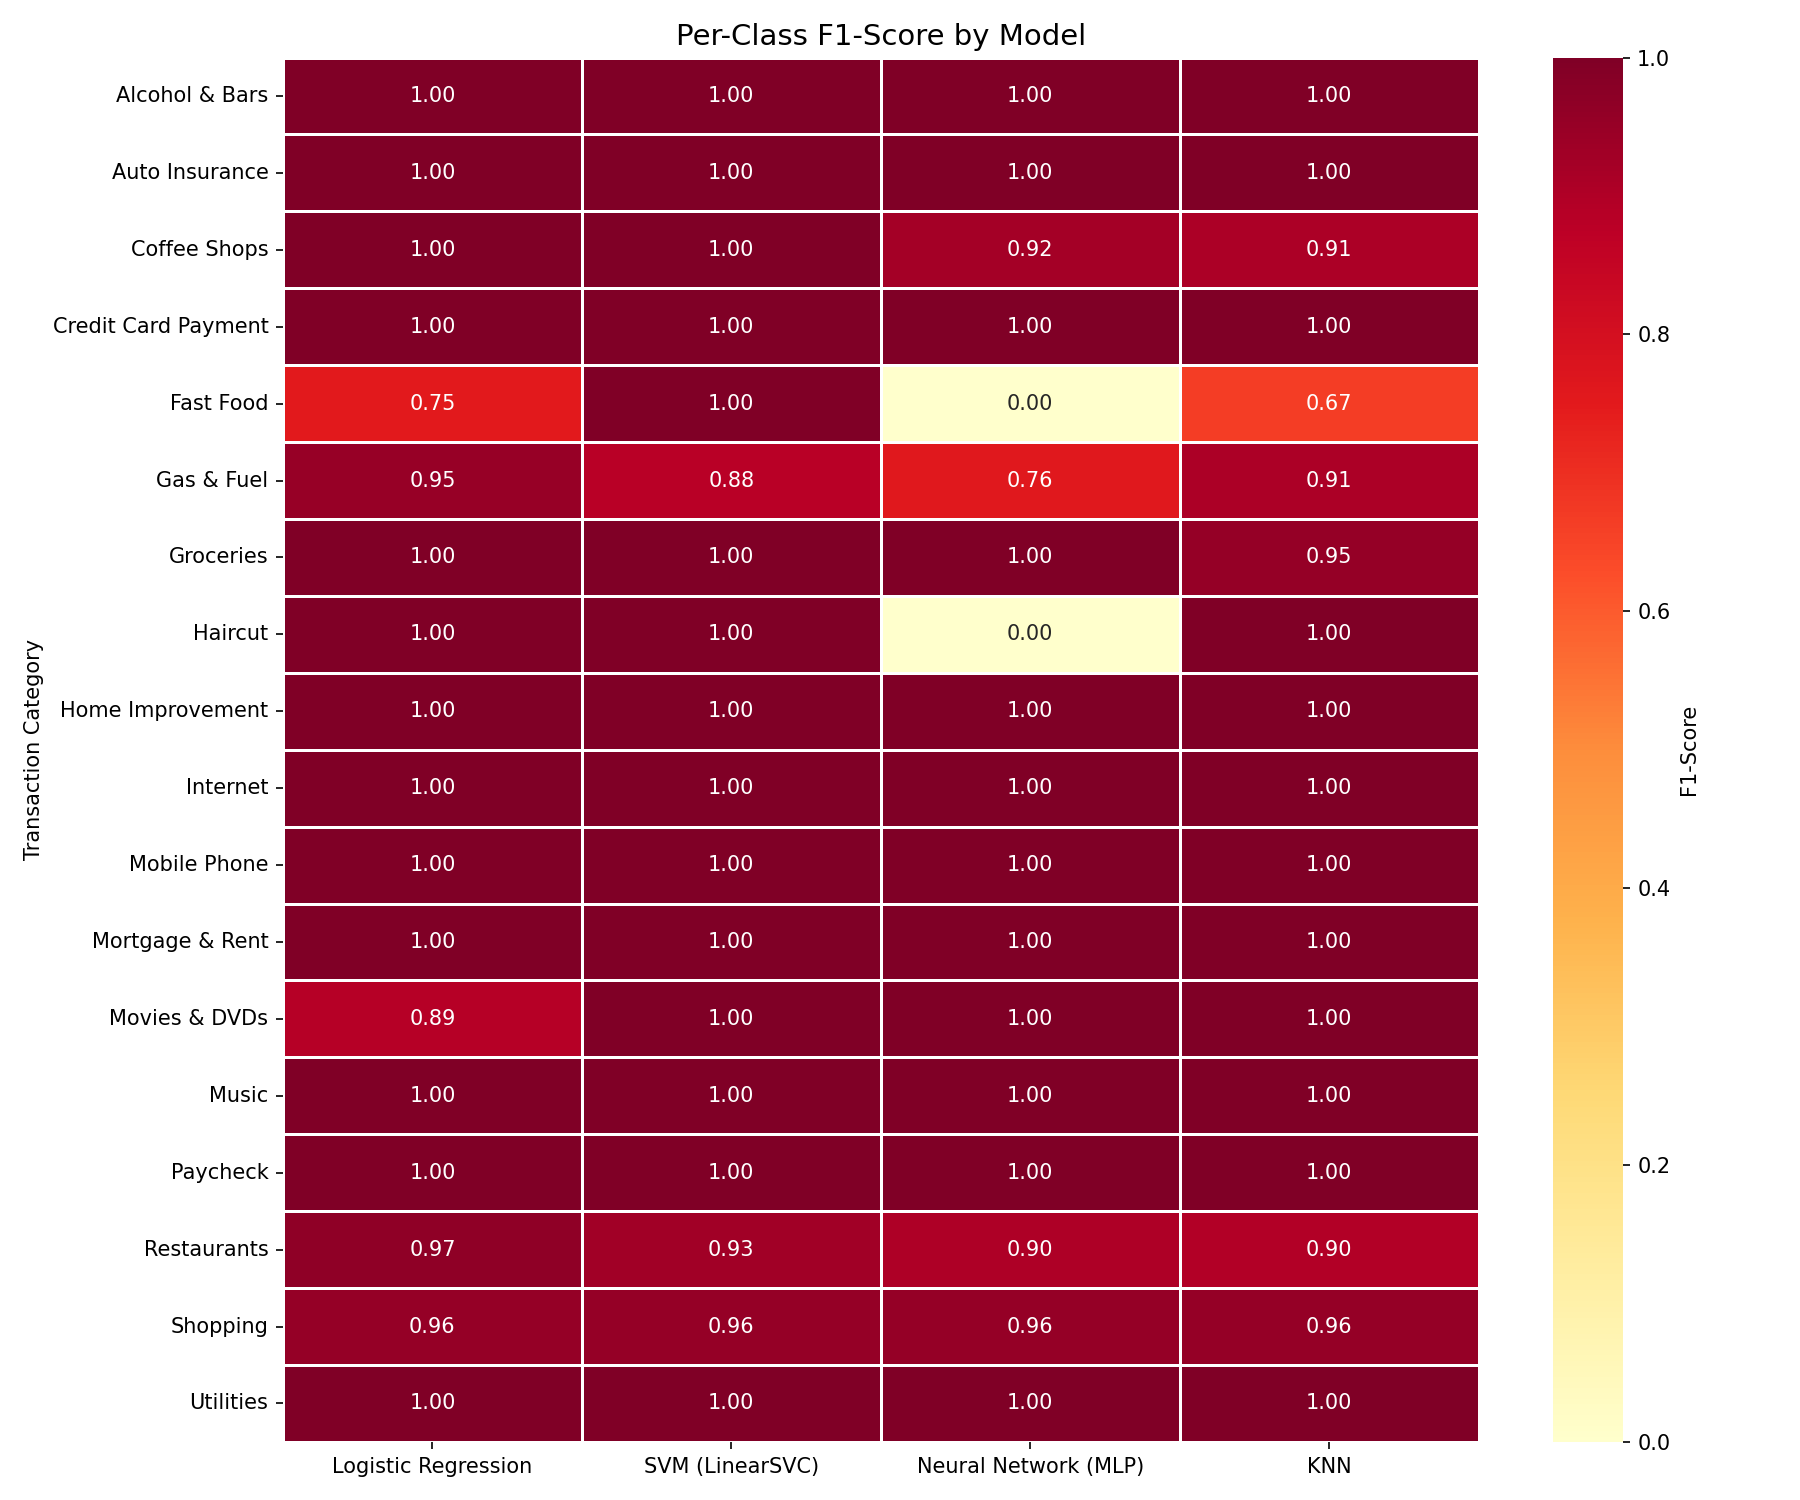
\includegraphics[width=0.85\textwidth]{per_class_f1_heatmap.png}
  \caption{Per-class F1-score heatmap. Darker red indicates lower performance. Gas \& Fuel and Restaurants show the most variation across models.}
  \label{fig:heatmap}
\end{figure}

The MLP training curve in Figure~\ref{fig:mlp_curve} shows the model converging quickly and the early stopping triggering before the maximum 500 epochs.

\begin{figure}[H]
  \centering
  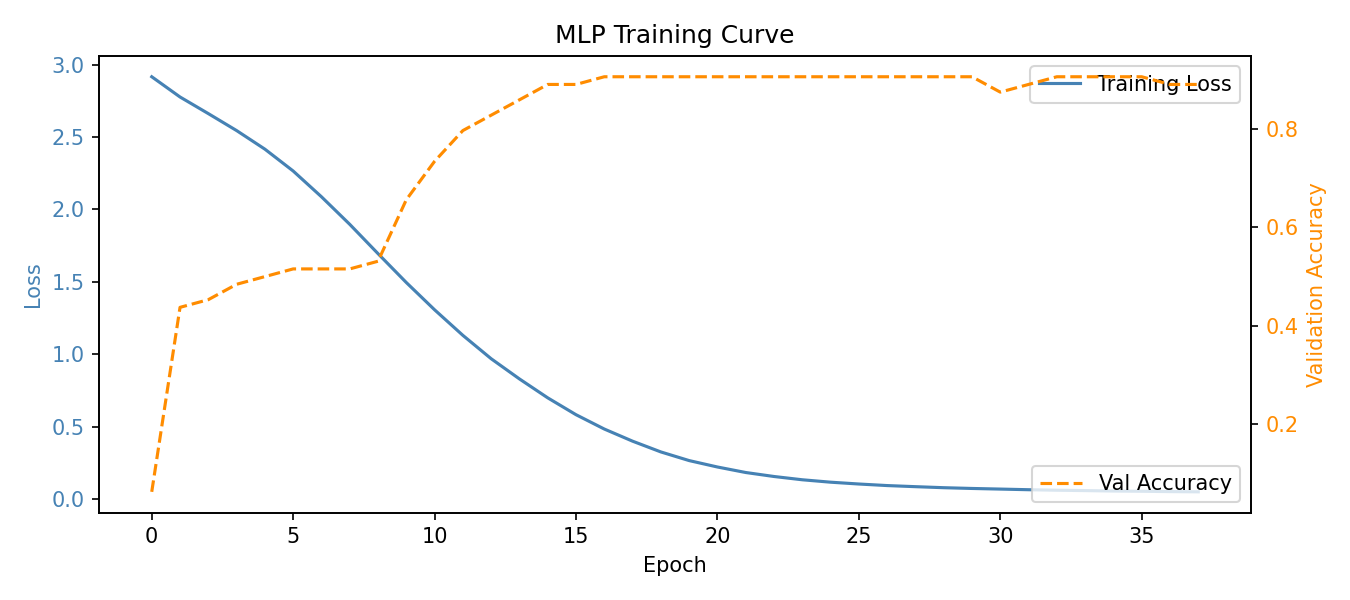
\includegraphics[width=0.65\textwidth]{mlp_training_curve.png}
  \caption{MLP loss and validation accuracy over training epochs. Early stopping halts training when validation accuracy stops improving.}
  \label{fig:mlp_curve}
\end{figure}

\section{Discussion}

\subsection{Why Linear Models Win}

Both Logistic Regression and SVM reached 98.1\% accuracy, which is notably higher than MLP (94.3\%) and KNN (96.2\%). The main reason is how distinctive the transaction descriptions are. Merchants like ``Starbucks'', ``Netflix'', ``Mortgage Payment'', and ``Biweekly Paycheck'' have almost no overlap across categories. Once these terms are represented as TF-IDF features, the class boundaries in that feature space are close to linear, and Logistic Regression and SVM can exploit that directly.

Inspecting the LR coefficients confirms this. The top predictive tokens for each class are exactly the merchant names you would expect: ``netflix'' and ``amazon video'' drive Movies \& DVDs, ``starbucks'' drives Coffee Shops, ``mortgage'' drives Mortgage \& Rent, and so on. The model is essentially doing pattern matching in a principled way.

MLP, on the other hand, needs enough data to learn useful non-linear feature interactions. With only 632 training samples, it does not have much to work with. It performs reasonably well (94.3\%) but cannot match the linear models.

\subsection{Challenging Categories}

Gas \& Fuel has the lowest F1 across most models. Looking at the confusion matrix, some Gas \& Fuel transactions get misclassified as Utilities. This makes sense: descriptions like ``Gas Company'' and ``Power Company'' look similar in TF-IDF space, and both are mid-range debit transactions from the Checking account.

Restaurants, Fast Food, and Alcohol \& Bars also show occasional confusion with each other. Venue names like ``Roadside Diner'', ``Brewing Company'', and ``American Tavern'' share some n-gram overlap, and the distinction between a restaurant and a bar is not always obvious from the description alone.

\subsection{Strengths and Weaknesses by Model}

\begin{itemize}
  \item \textbf{Logistic Regression}: Best F1, fully interpretable, very fast. The go-to choice for this kind of task.
  \item \textbf{SVM (LinearSVC)}: Nearly identical performance to LR with shorter training time. Less interpretable since it does not output probabilities.
  \item \textbf{MLP}: Lowest performance here due to data size constraints, but would likely improve with a larger dataset. Only model that can capture non-linear feature interactions.
  \item \textbf{KNN}: No training time (it stores the data), decent accuracy, but prediction is slow at scale since it requires computing distances to all training points. Also sensitive to the imbalance since \texttt{class\_weight} cannot be applied.
\end{itemize}

\subsection{Limitations}

The biggest limitation of this project is the dataset size. The labeled portion of the dataset has only 806 rows, of which 791 are usable. This is quite small for machine learning, and it limits how much we can trust comparisons between models. The fact that the test set only has 159 samples means that a few misclassifications have a big impact on the reported metrics.

The transaction descriptions in this dataset are also relatively clean and standardized. Real bank transaction strings are messier, often containing truncated merchant names, location codes, and transaction IDs (e.g., ``SQ *STARBUCKS \#1234 SEATTLE WA''). A model trained on this data would likely not transfer directly to a real banking application.

We also did not use date-based features. The day of the week or the time of month could help classify recurring charges like subscriptions and mortgage payments.

\section{Conclusion}

We built a financial transaction classification system using four machine learning models and a feature pipeline combining TF-IDF, normalized transaction amounts, and one-hot categorical features. Logistic Regression achieved the best performance at 98.1\% accuracy and a weighted F1-score of 0.9827, followed closely by SVM at 0.9817. MLP and KNN performed well given the small dataset but lagged behind the linear models.

The main takeaway is that when class-specific vocabulary is distinctive enough, TF-IDF with a linear classifier is a strong and efficient approach. More complex models like MLP did not add value here, but would be worth revisiting with a larger labeled dataset.

For future work, we would like to test on a larger and messier dataset, experiment with pre-trained text embeddings (e.g., sentence-transformers), and explore whether adding temporal features improves classification for recurring transactions.

\section{Individual Contributions}

\begin{itemize}
  \item \textbf{Ian Hock}: Feature engineering pipeline (TF-IDF, log-scaling, one-hot encoding, sparse feature matrix), Neural Network (MLP) implementation, Methodology sections 2.2 and 2.4.3.
  \item \textbf{Jaden Ong}: Data preprocessing pipeline (filtering, deduplication, normalization, rare category removal), SVM (LinearSVC) implementation and hyperparameter tuning, Methodology sections 2.1 and 2.4.2.
  \item \textbf{Justin Pelak}: KNN implementation and hyperparameter tuning, comparative analysis and all evaluation visualizations (confusion matrices, F1 heatmap, model comparison charts), Results section.
  \item \textbf{Sawyer Jones}: Data loading and exploratory analysis, Logistic Regression implementation and coefficient interpretability analysis, Introduction, Discussion, and Conclusion sections.
\end{itemize}

All members collaborated on model selection decisions, reviewed each other's results, and contributed to editing the final report.

\begin{thebibliography}{9}

\bibitem{dataset}
Noble David, S. Personal Transactions Dataset.
Kaggle, 2023.
\url{https://www.kaggle.com/datasets/shyakanobledavid/personal-transactions-userid-new-transactions/data}

\bibitem{sklearn}
Pedregosa, F. et al.
Scikit-learn: Machine Learning in Python.
\textit{Journal of Machine Learning Research}, 12:2825--2830, 2011.

\bibitem{tfidf}
Ramos, J.
Using TF-IDF to Determine Word Relevance in Document Queries.
\textit{Proceedings of the First Instructional Conference on Machine Learning}, 2003.

\bibitem{linearSVC}
Fan, R., Chang, K., Hsieh, C., Wang, X., and Lin, C.
LIBLINEAR: A Library for Large Linear Classification.
\textit{Journal of Machine Learning Research}, 9:1871--1874, 2008.

\bibitem{mlp}
Glorot, X. and Bengio, Y.
Understanding the difficulty of training deep feedforward neural networks.
\textit{Proceedings of AISTATS}, 2010.

\end{thebibliography}

\end{document}
